\documentclass[a4paper,14pt]{report} %размер бумаги устанавливаем А4, шрифт 14пунктов
\usepackage [utf8x] {inputenc} %включаем свою кодировку
\usepackage [T2A] {fontenc}
\linespread{1.3} %полуторный межстрочный интервал
\usepackage[english,russian]{babel}%используем русский и английский языки с переносами
\usepackage[final]{graphicx} 
\graphicspath{{images/}}%путь к рисункам
\usepackage[left=3cm,right=2cm,top=2cm,bottom=2cm,bindingoffset=0cm]{geometry}
\renewcommand\contentsname{Projects List} %%% renaming the Table of Contents

\begin{document}
\begin{titlepage}

\begin{center}   
{\bfseries  
ФЕДЕРАЛЬНОЕ ГОСУДАРСТВЕННОЕ АВТОНОМНОЕ ОБРАЗОВАТЕЛЬНОЕУЧРЕЖДЕНИЕ ВЫСШЕГО ОБРАЗОВАНИЯ,САНКТ-ПЕТЕРБУРГСКИЙ НАЦИОНАЛЬНЫЙ ИССЛЕДОВАТЕЛЬСКИЙ УНИВЕРСИТЕТ ИНФОРМАЦИОННЫХ ТЕХНОЛОГИЙ,МЕХАНИКИ И ОПТИКИ
\par\smallskip
Факультет Компьютерных технологий и управления
\par\smallskip
Кафедра Вычислительной техники\\
}
\par\smallskip
\mbox{Направление подготовки (специальность): 09.03.04 - «Программная инженерия»}

\vspace{3cm} 
{\bfseries
ОТЧЕТ 
\par\medskip
по практике
}
\end{center}  

\par\noindent \smallskip
{\bfseries Тема задания:}
\par\noindent \smallskip
{\bfseries Студент: } Игнатьева Ю.В. {\bfseries Группа: } P3311
\par\noindent \smallskip
{\bfseries Руководитель практики: } Соснин Владимир Валерьевич
\par\noindent \smallskip
{\bfseries Оценка, рекомендуемая руководителем: \line(1,0){75} \quad \line(1,0){75}}
\vspace{1cm}

\parindent=8cm
{\bfseries Практика пройдена с оценкой : \line(1,0){85} \par \bigskip
Подписи членов комиссии \par \bigskip

\begin{flushright}  
\line(1,0){100}(\line(1,0){100}) \par \bigskip
\line(1,0){100}(\line(1,0){100}) \par \bigskip
\line(1,0){100}(\line(1,0){100}) \par \bigskip
\end{flushright} 

\parindent=8cm
Дата \line(1,0){100} }
\vspace{\fill}
\begin{center}  
\bfseries Санкт-Петербург \par 2016
\end{center} 

\end{titlepage}% это титульный лист
\tableofcontents % это оглавление, которое генерируется автоматически
\chapter{Система компьютерной вёрстки TeX (LaTeX)}
\section{Краткое описание LaTeX}
В 1978 году профессор Гарвардского университета Дональд Кнут опубликовал первую версию систему для верстки текстов, которая ныне известна как TeX.  Кнут писал TeX во времена появления цифрового печатающего оборудования, чтобы изучить его потенциал и, в особенности, обратить тенденцию ухудшения типографского качества, которую он наблюдал на примере его собственных книг. TeX произносится как "тех". Последняя буква X в названии TeX — вовсе не английская буква "икс" (x), а греческая "хи". TeX считается наиболее качественной системой подготовки текстов. Как сказано в словаре компьютерных терминов (Douglas Downing and Michael A. Covington. Dictionary of Computer and Internet Terms. 8th ed. Barron's Educational Series. New York: Woodbury, 2003.) TeX определяет стандарт, к которому пытаются приблизиться другие настольные издательские системы.
\par
В начале восьмидесятых годов XX века Лесли Лампорт разработал систему LaTeX, которая была основана на форматирующих средствах TeX'а. LaTeX - макропакет, который позволяет при помощи уже заранее определенных, профессиональных макетов верстать авторам их работы с высоким типографским качеством. LaTeX произносится как "латех". Чтобы пользоваться системой LaTeX и создавать удобные для чтения текстовые произведения, совсем не надо быть умелым пользователем системы ТеХ - достаточно выбрать готовый стиль и использовать несколько простых команд в зависимости от того, что нужно в данном случае. Набор макросов, для решения задач, пополнялся с каждым годом, поэтому в 1992 году был организован файловый архив CTAN. CTAN - это акроним "Comprehensive TeX Archive Network". Будучи распространяемым под лицензией LaTeX Project Public License, LaTeX относится к свободному программному обеспечению.
\par
Главная идея LaTeX состоит в том, что теперь пользователь может сконцентрировать свои усилия на содержании и структуре текста, о том, что он напишет, не заботясь о деталях его оформления. Готовя свой документ, автор указывает логическую структуру текста (разбивая его на главы, разделы, таблицы, изображения), а LaTeX решает вопросы его отображения. Так содержание отделяется от оформления. Оформление при этом или определяется заранее (стандартное), или разрабатывается для конкретного документа. В конце девяностых годов XX века такая идея отделения содержания от оформления нашла своё продолжение в XML - расширяемом языке разметки (eXtensible Markup Language).
\par
В России TeX и LaTex появились в конце восьмидесятых годов, тогда же был разработан алгоритм автоматического переноса русских слов. 
\par
Пакет позволяет автоматизировать многие задачи набора текста и подготовки статей, включая
\begin{enumerate} %перечень
\item набор текста на нескольких языках;
\item нумерацию разделов и формул;
\item перекрёстные ссылки;
\item размещение иллюстраций и таблиц на странице;
\item генерацию оглавлений, списков иллюстраций и таблиц;
\item генерацию предметных указателей;
\item ведение библиографии и др.
\end{enumerate}

\section{Перечень сильных и слабых сторон TeX}
Перечислим основные достоинства TeX:
\begin{enumerate} %перечень
\item LaTeX предоставляет удобные и гибкие средства, чтобы напечатанный вами текст был "совсем как в книге". В частности, указав с помощью простых средств логическую структуру текста, автор может не вникать в детали оформления. Но при необходимости, эти детали могут быть изменены;
\item высокое качество и гибкость верстки абзацев и математических формул;
\item TeX неприхотлив к используемой технике. Например, им можно пользоваться на компьютерах на базе 80286-процессора;
\item TeXовские файлы обладают высокой степенью переносимости. TeX чрезвычайно мобилен и свободно доступен, поэтому система работает практически на всех существующих платформах.
\end{enumerate}

\noindent Однако, есть у TeXа и недостатки:
\begin{enumerate} %перечень
\item TeX работает относительно медленно, занимает много памяти;
\item некоторые пользователи, которые привыкли работать с редакторами наподобие Chiwriter, относят к недостаткам TeXа тот факт, что он не является системой типа WYSIWYG, то есть работа с исходным текстом и просмотр того, как текст будет выглядеть на печати, - разные операции. Но с другой стороны, благодаря этой особенности TeX время на подготовку текста сокращается;
\item переносимость TeXовских текстов снижается, если в них предусмотрен импорт графических файлов;
\item хотя предопределенные макеты имеют множество настраиваемых параметров, создание нового макета документа не очень простое дело и может занять много времени;
\item очень сложно писать неструктурированные и неорганизованные документы.
\end{enumerate}

Не смотря на то, что недостатков получилось больше, преимущества TeX позволяют ему быть популярным среди пользователей, существовать для всех типов компьютеров и применяться для подготовки как одностраничных писем, так и многотомных фолиантов. Многие редакции научных журналов рекомендуют, а иногда и вынуждают готовить статьи в системе LaTeX, чтобы потом, заменив всего лишь одно слово в названии класса печатного документа в преамбуле входного файла, издатель мог придать тексту тот облик, который отличает выбранный журнал.
\section{Инструмент для редактирования TeX - TeXworks}
Для редактирования отчета мной была выбрана свободная среда для работы с TeX-документами, включающая редактор, просмотрщик PDF - TeXworks, обладающая простым интерфейсом. TeXworks является удобным в использовании графическим интерфейсом (GUI) к системе подготовки документов TeX/LaTeX и других. Разработчик данного редактораДжонатан Кью. В комплект TeXworks включен набор шаблонов для создания наиболее часто используемых документов. Редактор включает в себя базовые возможности (характерные для большинства редакторов текста), систему автодополнения команд, запуск вёрстки и возможность добавления сценариев для преобразования текста документа. 
\par
Этот редактор был мной выбран, так как он идеально подходит при необходимости получить PDF файл в результате вёртки (используется pdfTeX). Для предварительного просмотра скомпилированных документов имеется интегрированный просмотрщик PDF (основанный на библиотеке Poppler), поддерживающий синхронизацию с исходным документом.
\chapter{Система контроля версий Git}
\section{Краткое описание Git}
Чтобы хранить и регистрировать изменения в файле с отчетом по практике, чтобы в дальнейшем была возможность вернуться к определённым старым версиям этого файла, мною была использована система контроля версий Git. Git (произносится как «гит») - распределённая система управления версиями, которая была создана Линусом Торвальдсом. Первая версия появилась в 2005 году. Очень много проектов используют Git, самые известные из них: ядро Linux, Android, MediaWiki, DokuWiki,  некоторые дистрибутивы Linux и другие. Программа является свободной. 

К особенностям реализации этой системы можно отнести то, что ядро Git представляет собой набор утилит командной строки с параметрами, а все настройки хранятся в текстовых файлах конфигурации. Такая реализация делает Git легко портируемым на любую платформу.

Репозиторий Git представляет собой каталог файловой системы, в котором находятся файлы конфигурации репозитория, файлы журналов, хранящие операции, выполняемые над репозиторием, индекс, описывающий расположение файлов и хранилище, содержащее собственно файлы. 
\section{Описание сильных и слабых сторон Git }
Сравнение Git другими системами контроля версий можно разделить на два этапа. 

Так как Git является распределенной системой контроля версий, в первую очередь сравним ее с "родственными" ей системами. Наиболее популярными и называемыми преимуществами Git перед другими системами являются:
\begin{enumerate} %перечень
\item высокая производительность;
\item продуманная система команд, позволяющая удобно встраивать git в скрипты;
\item качественный веб-интерфейс;
\item репозитории git могут распространяться и обновляться общесистемными файловыми утилитами архивации и обновления, такими как rsync;
\item Развитые средства интеграции с другими системами контроля версий, в частности, с CVS, SVN и Mercurial.
\end{enumerate}

В числе недостатков Git обычно называют:
\begin{enumerate} %перечень
\item некоторое неудобство для пользователей, переходящих с других систем. Команды Git, ориентированные на наборы изменений, а не на файлы, могут вызвать недоумение у пользователей, привыкших к файл-ориентированным системам контроля версий, таким как SVN;
\item большие затраты времени, по сравнению с файл-ориентированными системами, на формирование истории конкретного файла, истории правок конкретного пользователя, поиска изменений, относящихся к заданному месту определённого файла;
\item большие накладные расходы при работе с проектами, в которых делаются многочисленные несвязанные между собой изменения файлов;
\item система работает только с файлами и их содержимым, и не отслеживает пустые каталоги.
\end{enumerate}

Во-вторых, сравним систему Git с централизованными системами управления версиями (такими как, например, Subversion).
Основные преимущества распределённых систем - их гибкость и значительно большая (по сравнению с централизованными системами) автономия отдельного рабочего места. Каждый компьютер разработчика является, фактически, самостоятельным и полнофункциональным сервером, из таких компьютеров можно построить произвольную по структуре и уровню сложности систему, задав (как техническими, так и административными мерами) желаемый порядок синхронизации. При этом каждый разработчик может вести работу независимо, так, как ему удобно, изменяя и сохраняя промежуточные версии документов, пользуясь всеми возможностями системы (в том числе доступом к истории изменений) даже в отсутствие сетевого соединения с сервером. Связь с сервером или другими разработчиками требуется исключительно для проведения синхронизации, при этом обмен наборами изменений может осуществляться по различным схемам.

К недостаткам распределённых систем можно отнести увеличение требуемого объёма дисковой памяти: на каждом компьютере приходится хранить полную историю версий, тогда как в централизованной системе на компьютере разработчика обычно хранится лишь рабочая копия, то есть срез репозитория на какой-то момент времени и внесённые изменения. Менее очевидным, но неприятным недостатком является то, что в распределённой системе практически невозможно реализовать некоторые виды функциональности, предоставляемые централизованными системами. Это:
\begin{enumerate} %перечень
\item блокировка файла или группы файлов (для хранения признака блокировки нужен общедоступный и постоянно находящийся в онлайне центральный сервер);
\item слежение за определённым файлом или группой файлов (изменения файлов происходят на разных серверах, слияния и выделения ветвей происходят локально, об изменениях становится известно только при синхронизации, причём не всем разработчикам, а только тем, кто в данной синхронизации участвует);
\item единая сквозная нумерация версий системы и/или файлов, в которой номер версии монотонно возрастает (такая нумерация также требует наличия главного сервера, задающего номера версий для всех остальных);
\item локальная работа пользователя с отдельной, небольшой по объёму выборкой из значительного по размеру и внутренней сложности хранилища на удалённом сервере.
\end{enumerate}

С момента рождения в 2005 году Git развивался и эволюционировал, становясь проще и удобнее в использовании, сохраняя при этом свои первоначальные качества. Он невероятно быстр, очень эффективен для больших проектов, а также обладает превосходной системой ветвления для нелинейной разработки.
\chapter{Литература}
Цель практики - найти систему имитационного моделирования (СИМ), которая быстрее остальных умеет моделировать работы простейшей СМО М/М/1 с двумя видами приоритетов (ДОБП, ДООП) для двух классов заявок. Но перед выполнением практической части задания, надо подробно изучить каждую СИМ, которая будет использоваться. Первичный список СИМ: 
\begin{enumerate} %перечень
\item GPSS World;
\item Anylogic 7.1.
\end{enumerate}
Остальные системы будут рассматриваться после сравнения вышеперечисленных СИМ.
Для изучения системы AnyLogic мною была выбрана следующая литература:
\begin{enumerate} %перечень
\item А.Г. Куприяшкин "Основы моделирования систем". Учебное пособие посвящено моделированию динамических систем в среде AnyLogic. Показаны основные этапы разработки моделей – от постановки задачи до создания анимированной презентации.
\item В.Д. Боев "Концептуальное проектирование систем в Anylogic 7 и GPSS World". В этой книге предлагаются различные методики разработки имитационных моделей с применением инструментальных средств AnyLogic 7 и GPSS World.
\item В.Д. Боев  "Компьютерное моделирование. Пособие для практических занятий, курсового и дипломного проектирования в AnyLogic 7". В этом пособие предлагаются методики разработки имитационных моделей проектируемых систем с применением инструментальных средств AnyLogic 7. Приводятся сравнительные оценки результатов моделирования разнородных дискретных процессов, полученных на моделях одной и той же проектируемой системы в GPSS World и AnyLogic 7.
\item Ilya Grigoryev "AnyLogic 7 in Three Days: A Quick Course in Simulation Modeling".
\end{enumerate}
Для изучения GPSS World я буду использовать уже упомянутые книги В.Д.Боева, а так же: 
\begin{enumerate} %перечень
\item Томашевский В.Н., Жданова Е.Т. "Имитационное моделирование в среде GPSS".
\item Алиев Т.И. "Основы моделирования дискретных систем".
\end{enumerate}
Кратко перескажем основные моменты из прочитанных книг.

\section{А.Г. Куприяшкин}
Учебное пособие А.Г. Куприяшкина "Основы моделирования систем" содержит шесть разделов, материал которых разбит на параграфы. 

В первом разделе расписаны основные понятия, которые могут вызывать затруднения у академической аудитории, например, что такое адекватность модели (это соответсвтиве модели оригиналу, характеризуемое степенью близости свойств модели свойствам исследуемой системы),  верификация (т.е. проверка достоверности модели), валидация (это процесс, позволяющий установить, является ли модель точным представлением системы для конкретных целей исследования) и т.д. Так же в этом разделе привидены методы для построения математических моделей, задачи моделирования, направления и инструменты моделирования. Вся информация этого раздела даст неподготовленному читателю представление о понятии моделирования и о его целях. 

Во втором разделе "Основ моделирования систем" подробно описывается среда инструмент имитационного моделирования AnyLogic. Инструмент обладает современным графическим русскоязычным интерфейсом и позволяет использовать язык Java для разработки моделей. Автор подробно, начиная от регистрации на сайте компании и установки, показывает с помощью понятного материала и изображений этапы работы в данной среде, рассказывает про каждый элемент интерфейса, помогает создать нам наш собственный первый проект. В результате появляется представление о том, как надо планировать проект, для чего нужно формулировать его задачу, разделять его изначально на этапы.

В третьем раздаеле говорится о детерминированных непрерывных системах. В первом параграфе этого раздела автор приводит основные сведения, что учитывается при моделировании физических систем, описывает четыре режима (стационарный, переходный, периодический, динамический) динамики системы и объясняет все это на простой модели реактора идеального смешения.  Далее автор предлагает нам в качестве примера построить имитационную модель пружинного маятника, эту задачу он делит на два этапа: математическую ("формализованную") и имитационную интерактивную ("неформализованную"). Затем добавляем в модель трехмерную анимацию. В AnyLogic
она отображается в специальных окнах. В результате создалась интерактивная модель, оснащенная элементами 2D–3D-визуализации, средствами навигации и управления. Существует область задач, когда параметры системы изменяются по времени и пространственным координатам. Для таких систем создаются модели с распределенными параметрами, которые так же затрагиваются автором в этом разделе. В конце этого раздела А.Г. Куприяшкин формулирует обратную задачу моделирования, которая сводится к нахождению таких значений параметров модели, которые бы соответствовали определенному состоянию системы, и её решение.

Четвертый раздел посвящен дискретно-событийному моделированию. Здесь рассматриваются системы, которые обладают разнообразным поведением, и в зависимсоти от входных сигналов или событий переходят в разные состояния, даётся понятие "конечный автомат" (математическая модель поведения устройств с конечной памятью), а так же приводится пример реализации по-настоящему культовой игры "Жизнь".

В последней главе автор пишет о моделировании систем массового обслуживания. В первую очередь, он дает определения основным понятиям, связанным с системами массового обслуживания(СМО), а затем показывает все на понятном примере с моделированием процесса выполнения задач компьютером. 

В конце книги есть вопросы и задания на моделирование, где можно проверить понимание темы, а так же есть библиографический список с перечнем рекомендуемой автором, а так же используемой в книге, литературой. Эта книга предназначена как для академической, так и для профессиональной аудитории. В частности, опыт и знания, полученные при реализации в AnyLogic различных примеров моделей, помогут мне при сравнении Anylogic с другими системами имитационного моделирования.

\section{В.Д. Боев}
"Концептуальное проектирование систем в Anylogic 7 и GPSS World" написано в виде курса для дистационного обучения. Курс предназначен для проведения практических занятий по дисциплинам, связанным с проектированием и компьютерным моделированием систем с использованием систем имитационного моделирования, и рассчитан на 16 часов. 

Курс разбит на девять лекций, в каждой из которых рассматриваются пример модели, реализованный как в AnyLogic, так и в GPSS. Для первой лекции выбрана модель несложная и понятная многим: модель обработки запросов сервером. В последующих лекциях рассматриваются модели процесса изготовления в цехе деталей, функционирования направления связи, функционирования сети связи, функционирования системы связи, функционирования предприятия, предоставления ремонтных услуг, функционирования системы воздушных перевозок и обработки документов в организации. Автор подробно расписал все этапы, начиная с постановки задачи, а в первых лекциях даже сделал акценты на самих инструментах имитационного моделирования GPSS и AnyLogic для людей, которые работают с этими программами в первый раз. Последние лекции рассчитаны на людей, прошедших весь курс, либо на профессиональную аудиторию. 

За этот день я проработала все эти модели, последние из них смоделировала в AnyLogic за исключением анимации, ведь по индивидуальному заданию модели в разных СИМ должны работать без визуализации моделирования.

Учебное пособие В.Д. Боева "Компьютерное моделирование. Пособие для практических занятий, курсового и дипломного проектирования в AnyLogic 7" содержит ту же информацию, но оформлено в виде книги.

\section{С.М. Щербаков}
Для изучения одного из наиболее распространенного инструмента имитационного моделирования Arena я выбрала учебное пособие Щербакова С.М. "Имитационное моделирование экономических процессов в системе Arena: Учебное пособие". Как и в предыдущих пособиях основной упор сделан на примеры, которые будут понятны всем (например, клиенты в парикмахерской), а также в данной книге много изображений, расположенных по порядку, помогающих новичку понять, куда стоит нажать, что надо написать и так далее. В самом начале автор рассказывает об основных понятиях, что имитационная модель представляет собой граф, узлами которого являются модули, последние в свою очередь связаны между собой с помощью соединений, по которым между модулями перемещаются транзакты(динамические объекты имитационной модели), и что модель в системе Arena является процессно-ориентированной. Далее автор показывает, где можно создать переменную, как изменить ее значение, где можно создать ресурсы и задать их количество, как изменить настройки очереди и дисциплины обслуживания, рассказывает про базовые модули:
\begin{enumerate} %перечень
\item Create (генератор транзактов);
\item Dispose (терминатор транзактов);
\item Process (обработка, действие);
\item Decide (ветвление);
\item Assign (присвоение значений переменным модели и атрибутам транзакта, проходящего через модуль);
\item Hold (выполняет роль «шлагбаума»);
\item Batch (объединение (временное или постоянное) заданного числа транзактов в один транзакт);
\item Match (синхронизация двух или более (до пяти) транзактов) 
\end{enumerate}

В книге есть глава про анимацию и визуализацию моделей, но для выполнения работы нам это не понадобится.
\section{Simulink}
Для ознакомления с графическая средой имитационного моделирования Simulink я воспользовалась документацией по SimEvents http://www.mathworks.com/help/simevents/index.html, а именно разделами Modeling, в котором рассказано про основные функции и блоки, про настройки этих блоков (значения всех параметров), про входные и выходные порты блоков, а так же разделом Simulation, где расписаны настройки моделирования, как получить результаты работы модели, отладка моделирования, анализ сигналов и событий.


\chapter{Выполнение индивидуального задания}
\section{Описание моделей СМО}
Для выполнения работы нужно создать модели СМО М/М/1 с двумя видами приоритетов (ДОБП, ДООП) для двух классов заявок. 

Обозначение СМО M/M/1  в символике Кендалла значит, что:
\begin{enumerate} %перечень
\item интервалы времени между моментами поступления заявок в систему распределены по экспоненциальному (показательному) закону;
\item длительность обслуживания заявок в приборе распределена по экспоненциальному (показательному) закону;
\item один обслуживающий прибор в системе;
\item накопитель - неограниченной ёмкости.
\end{enumerate}

Бесприоритетная дисциплина обслуживания (ДО БП) - это дисциплина обслуживания, при которой заявки выбираются на обслуживание в порядке поступления.

Дисциплина обслуживания с относительными приоритетами (ДО ОП) - это дисциплина обслуживания, при которой поступление в систему заявки с более высоким приоритетом по сравнению с обслуживаемой в приборе не приводит к прерыванию обслуживания, но при выборе заявки на обслуживание, выбирается заявка с наибольшим приоритетом. 

\begin{figure}[h] %определить место рисунка в тексте
\center{\includegraphics[width=0.5\linewidth]{model}}
\caption{Схема разработанной модели}
\label{ris:model}
\end{figure} %вставить ссылку на рисунок

\section{Система GPSS World}
\subsection{Описание системы проектирования}
Из всех разработанных языков моделирования, ни один не имел большего влияния, чем GPSS - Универсальная Система Моделирования (General Purpose Simulation System). Впервые разработанная сотрудником IBM Джеффри Гордоном в начале 1960-х, GPSS является одним из наиболее популярных в мире языков моделирования.

GPSS World является объектно-ориентированным языком. Его возможности визуального представления информации позволяют наблюдать и фиксировать внутренние механизмы функционирования моделей. Его интерактивность позволяет одновременно исследовать и управлять процессами моделирования. С помощью встроенных средств анализа данных можно легко вычислить доверительные интервалы и провести дисперсионный анализ.

Модель (программа) на языке GPSS представляет собой последовательность операторов (их называют блоками), отображающих события, происходящие в СМО при перемещениях транзактов. Поскольку в интерпретаторах GPSS реализуется событийный метод и в СМО может быть одновременно много транзактов, то интерпретатор будет попеременно исполнять разные фрагменты программы, имитируя продвижения транзактов в текущий момент времени до их задержки в некоторых устройствах или очередях.

\subsection{Создание моделей СМО в GPSS}
Для начала создадим модель СМО, показанную на Рис.~\ref{ris:model}, в GPSS.

Для ДО БП:\par\noindent
TRA1	VARIABLE	Exponential(1,0,10) \par\noindent
TRA2	VARIABLE	Exponential(2,0,10) \par\noindent
TOB1	VARIABLE	Exponential(3,0,1) \par\noindent
TOB2	VARIABLE	Exponential(4,0,1)  \par              
GENERATE	V\$TRA1 ;генерирование заявок 1-го класса (загрузка = 0.1)\par 
ASSIGN 	time1,V\$TOB1 \par
TRANSFER ,begin1 \par
GENERATE	V\$TRA2 ;генерирование заявок 2-го класса (загрузка = 0.1)\par 
ASSIGN 	time1,V\$TOB2 \par
TRANSFER ,begin1 \par\noindent
begin1	QUEUE	Queue1 \par
SEIZE 	Uzel \par
DEPART	Queue1 \par
ADVANCE 	P\$time1 \par
RELEASE 	Uzel \par
TERMINATE 1 \par
\vspace{0.5cm} 
Модель с относительными приоритетами почти не отличается от вышенаписанной модели с бесприоритетной дисциплиной обслуживания, только при генерации заявок второго класса приоритет будет задаваться равным 2 вручную, а не равным 1 по умолчанию, чтобы при выборе заявки на обслуживание, выбиралась заявка второго класса(если хотя бы одна из них есть в системе), т.е. заявка с большим приоритетом:\par\noindent
TRA1	VARIABLE	Exponential(1,0,10) \par\noindent
TRA2	VARIABLE	Exponential(2,0,10) \par\noindent
TOB1	VARIABLE	Exponential(3,0,1) \par\noindent
TOB2	VARIABLE	Exponential(4,0,1)  \par              
GENERATE	V\$TRA1 \par 
ASSIGN 	time1,V\$TOB1 \par
TRANSFER ,begin1 \par
GENERATE	V\$TRA2,,,,2 \par 
ASSIGN 	time1,V\$TOB2 \par
TRANSFER ,begin1 \par\noindent
begin1	QUEUE	Queue1 \par
SEIZE 	Uzel \par
DEPART	Queue1 \par
ADVANCE 	P\$time1 \par
RELEASE 	Uzel \par
TERMINATE 1 \par
\subsection{Замеры времени моделирования в GPSS}
В процессе замеров времени было проведено девять независимых экспериментов для каждой СМО: для разных соотношений загрузки классов (0.1+0.1, 0.3+0.3, 0.48+0.48), а также для разного количества пропущенных заявок ($10^6$, $5*10^6$, $10^7$).

\begin{table}[h!]
\caption{Результаты измерений СМО с ДО БП}
\begin{tabular}{|c|c|c|c|c|c|c|c|c|c|}
\hline
 & \multicolumn{3}{|c|}{1.000.000} & \multicolumn{3}{|c|}{5.000.000} & \multicolumn{3}{|c|}{10.000.000} \\
\hline
 & 0.1+0.1 & 0.3+0.3 & 0.48+0.48 & 0.1+0.1 & 0.3+0.3 & 0.48+0.48 & 0.1+0.1 & 0.3+0.3 & 0.48+0.48 \\
\hline
1 замер & 4 & 3 & 4 & 17 & 17 & 17 & 35 & 36 & 36  \\
\hline
2 замер & 4 & 4 & 3 & 18 & 18 & 17 & 36 & 35 & 37 \\
\hline
3 замер & 3 & 3 & 3 & 17 & 18 & 17 & 34 & 36 & 35 \\
\hline
4 замер & 3 & 3 & 3 & 17 & 17 & 17 & 35 & 39 & 36 \\
\hline
Ср.знач. & 3.5 & 3.25 & 3.25 & 17.25 & 17.5 & 17 & 35 & 36.5 & 35.75 \\
\hline
\end{tabular}
\end{table} 

Рассчитаем доверительный интервал для времён моделирования системы с количеством заявок, равным $10^6$, $5*10^6$, $10^7$ с доверительной вероятностью 95\%. Для этого выполним прогоны имитационной модели с разными соотношениями загрузок классов (0.1+0.1, 0.3+0.3, 0.48+0.48) при неизменных параметрах. Для каждого соотношения сделаем четыре прогона и найдем среднее значение.

\begin{table}[h!]
\caption{Доверительные интервалы измерений СМО с ДО БП}
\begin{tabular}{|c|c|c|c|c|c|}
\hline
 Количество заявок & Среднее значение & С.к.о. & Дов. вероятность & Дов. интервал & Результат\\
\hline
1.000.000 & 3.33 & 0.12 & 95\% & 0.29 & 3.33 ± 0.30 \\
\hline
5.000.000 & 17.25 & 0.20 & 95\% & 0.51 & 17.25 ± 0.51 \\
\hline
10.000.000 & 35.75 & 0.61 & 95\% &1.52 & 35.75 ± 1.53 \\
\hline
\end{tabular}
\end{table} 

Аналогично системе с бесприоритетной дисциплиной обслуживания выполним прогоны модели для СМО с относительными приоритетами.

\begin{table}[h!]
\caption{Результаты измерений СМО с ДО ОП}
\begin{tabular}{|c|c|c|c|c|c|c|c|c|c|}
\hline
 & \multicolumn{3}{|c|}{1.000.000} & \multicolumn{3}{|c|}{5.000.000} & \multicolumn{3}{|c|}{10.000.000} \\
\hline
 & 0.1+0.1 & 0.3+0.3 & 0.48+0.48 & 0.1+0.1 & 0.3+0.3 & 0.48+0.48 & 0.1+0.1 & 0.3+0.3 & 0.48+0.48 \\
\hline
1 замер & 3 & 4 & 4 & 18 & 18 & 18 & 38 & 37 & 38  \\
\hline
2 замер & 3 & 4 & 5 & 18 & 18 & 19 & 37 & 37 & 37 \\
\hline
3 замер &  4 & 4 & 3 & 19 & 20 & 18 & 38 & 38 & 37 \\
\hline
4 замер & 4 & 4 & 4 & 19 & 19 & 18 & 37 & 37 & 37 \\
\hline
Ср.знач. &  3.5 & 4 & 4 & 18.5 & 18.75 & 18.25 & 37.5 & 37.25 & 37.25 \\
\hline
\end{tabular}
\end{table} 

\begin{table}[h!]
\caption{Доверительные интервалы измерений СМО с ДО ОП}
\begin{tabular}{|c|c|c|c|c|c|}
\hline
 Количество заявок & Среднее значение & С.к.о. & Дов. вероятность & Дов. интервал & Результат\\
\hline
1.000.000 & 3.83 & 0.24 & 95\% & 0.59 & 3.83 ± 0.59 \\
\hline
5.000.000 & 18.50 & 0.20 & 95\% & 0.51 & 18.50 ± 0.51 \\
\hline
10.000.000 & 37.33 & 0.12 & 95\% &0.29 & 37.33 ± 0.30 \\
\hline
\end{tabular}
\end{table} 

\section{Система AnyLogic 7.1}
\subsection{Описание системы проектирования}
AnyLogic - программное обеспечение для имитационного моделирования сложных систем и процессов, разработанное российской компанией «Экс Джей Текнолоджис». Программа обладает графической средой пользователя и позволяет использовать язык Java для разработки моделей. Программный продукт предназначен для проектирования и оптимизации бизнес-процессов или любых сложных систем, таких как производственный цех, аэропорт, госпиталь и т.д. Инструмент поддерживает все методы бизнес моделирования - системную динамику, дискретно-событийное (процессное) и агентное моделирование. Основной упор в разработке продукта сделан на его гибкость и простоту использования для неопытных в создании моделей пользователей.

AnyLogic 7 - самое значительное обновление программы в течение 6 лет. По мнению разработчиков, этот релиз - большой шаг вперед в развитии продукта. Результат выразился в значительном упрощении и ускорении работы программы, расширении её функциональности.

Программный инструмент AnyLogic основан на объектно-ориентированной концепции. Другой базовой концепцией является представление модели как набора взаимодействующих, параллельно функционирующих активностей. Активный объект в AnyLogic - это объект со своим собственным функционированием, взаимодействующий с окружением. Он может включать в себя любое количество экземпляров других активных объектов.

Графическая среда моделирования поддерживает проектирование, разработку, документирование модели, выполнение компьютерных экспериментов, оптимизацию параметров относительно некоторого критерия. При разработке модели можно использовать элементы визуальной графики: диаграммы состояний, сигналы, события (таймеры), порты
и т.д.; синхронное и асинхронное планирование событий; библиотеки активных объектов.

\subsection{Создание моделей СМО в AnyLogic}
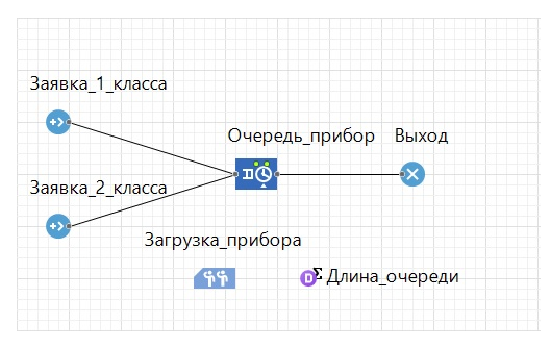
\includegraphics[width=0.5\linewidth]{model_AnyLogic}

Так как нам нужно создать полностью эквивалентные модели СМО в системах GPSS World и Anylogic (т.е. модели должны рассчитывать одинаковое количество характеристик и работать без визуализации моделирования), в AnyLogic дополнительно был написан код, который считает загрузку прибора, среднюю длину очереди и среднее время ожидания, а так же перед "прогоном" модели, чтобы повысить скорость выполнения, отключим графический интерфейс, для этого будем использовать простой эксперимент, а именно напишем в свойстве нашего эксперимента следующий код:\par
getEngine().setRealTimeMode( false );\par
getPresentation().getPanel().setFrameManagementAdaptive( false );\par
getPresentation().getPanel().setFrameRate( 0.1 );\par\noindent
который убирает анимацию при "прогоне" модели.

Для реализации ДО ОП был написан класс заявки, хранящий переменную, обозначающую приоритет. При создании заявки, эта переменная приравнивалась 1 или 2, в зависимости от класса заявки, а на обслуживание в приборе из очереди выбиралась заявка с большим приоритетом. 
\vspace{0.5cm} \par\noindent
public class Class2 extends com.anylogic.libraries.enterprise.Entity implements Serializable \{\par\noindent
public double time1;\par\noindent
public int type;\par\noindent
public double start\_waiting;\par\noindent
public Class2() \{\}\par\noindent
public Class2(double time1, int type) \{\par
this.time1 = time1;\par
this.type = type;\par\noindent
this.start\_waiting = start\_waiting;\par\noindent
\} \par\noindent
public double Start\_waiting()\{\par
return start\_waiting;\par\noindent
\}\par\noindent
public int Type()\{\par
return type;\par\noindent
\}\par\noindent
public double Time1()\{\par
return time1;\par\noindent
\}\par\noindent
@Override\par\noindent
public String toString() \{\par
return  \par
"time1 = " + time1 + \par
"type = " + type + \par
"start\_waiting =" + start\_waiting; \par
\}\par\noindent
\}\par

\subsection{Замеры времени моделирования в AnyLogic}
Количество экспериментов для СИМ AnyLogic аналогично системе GPSS World.

\begin{table}[h!]
\caption{Результаты измерений СМО с ДО БП}
\begin{tabular}{|c|c|c|c|c|c|c|c|c|c|}
\hline
 & \multicolumn{3}{|c|}{1.000.000} & \multicolumn{3}{|c|}{5.000.000} & \multicolumn{3}{|c|}{10.000.000} \\
\hline
 & 0.1+0.1 & 0.3+0.3 & 0.48+0.48 & 0.1+0.1 & 0.3+0.3 & 0.48+0.48 & 0.1+0.1 & 0.3+0.3 & 0.48+0.48 \\
\hline
1 замер & 15.9 & 16.1 & 16.3 & 70.9 & 64 & 64.4 & 115.5 & 113.7 & 128.5 \\
\hline
2 замер & 16.1 & 15.3 & 15.8 & 63.1 & 63.3 & 63.9 & 113 & 115.1 & 112.5 \\
\hline
3 замер & 13.9 & 15.8 & 17.1 & 64.5 & 61.3 & 64 & 112.6 & 124.9 & 108.6 \\
\hline
4 замер & 15.1 & 15.2 & 15.7 & 65.4 & 62.4 & 62.4 & 118.9 & 120.9 & 121.6 \\
\hline
Ср.знач. & 15.25 & 15.6 & 16.225 & 65.975 & 62.75 & 63.675 & 115 & 118.65 & 117.8 \\
\hline
\end{tabular}
\end{table} 

\begin{table}[h!]
\caption{Доверительные интервалы измерений СМО с ДО БП}
\begin{tabular}{|c|c|c|c|c|c|}
\hline
 Количество заявок & Среднее значение & С.к.о. & Дов. вероятность & Дов. интервал & Результат\\
\hline
1.000.000 & 15.69 & 0.40 & 95\% & 1.00 & 15.69 ± 1.01 \\
\hline
5.000.000 & 64.13 & 1.36 & 95\% & 3.37 & 64.13 ± 3.37 \\
\hline
10.000.000 & 117.15 & 1.56 & 95\% &3.87 & 117.15 ± 3.88 \\
\hline
\end{tabular}
\end{table} 

\begin{table}[h!]
\caption{Результаты измерений СМО с ДО ОП}
\begin{tabular}{|c|c|c|c|c|c|c|c|c|c|}
\hline
 & \multicolumn{3}{|c|}{1.000.000} & \multicolumn{3}{|c|}{5.000.000} & \multicolumn{3}{|c|}{10.000.000} \\
\hline
 & 0.1+0.1 & 0.3+0.3 & 0.48+0.48 & 0.1+0.1 & 0.3+0.3 & 0.48+0.48 & 0.1+0.1 & 0.3+0.3 & 0.48+0.48 \\
\hline
1 замер & 16.6 & 15.3 & 17.9 & 68.8 & 61.9 & 67.9 & 109.6 & 110.7 & 109.8  \\
\hline
2 замер & 14.5 & 15.5 & 13.3 & 63.1 & 64.8 & 66.3 & 108.8 & 112.5 & 110 \\
\hline
3 замер & 13.6 & 15.2 & 13 & 64.5 & 68.6 & 68.5 & 115.7 & 104 & 105.8  \\
\hline
4 замер & 14.2 & 15.5 & 15.2 & 65.4 & 69.5 & 66.4  & 113.2 & 115.5 & 111.6\\
\hline
Ср.знач. &  14.725 & 15.375 & 14.85 & 65.45 & 66.2 & 67.275 & 111.825 & 110.675 & 109.3 \\
\hline
\end{tabular}
\end{table} 

\begin{table}[h!]
\caption{Доверительные интервалы измерений СМО с ДО ОП}
\begin{tabular}{|c|c|c|c|c|c|}
\hline
 Количество заявок & Среднее значение & С.к.о. & Дов. вероятность & Дов. интервал & Результат\\
\hline
1.000.000 & 14.98 & 0.28 & 95\% & 0.70 & 14.98 ± 0.70 \\
\hline
5.000.000 & 66.31 & 0.75 & 95\% & 1.86 & 66.31 ± 1.87 \\
\hline
10.000.000 & 110.60 & 1.03 & 95\% &2.56 & 110.60 ± 2.57 \\
\hline
\end{tabular}
\end{table} 


\section{Система визуального проектирования имитационных моделей Arena}
\subsection{Описание системы проектирования}
Arena, разработанное компанией Systems Modeling Corporation программное обеспечение для имитационного моделирования, позволяет создавать подвижные компьютерные модели, используя которые можно адекватно представить очень многие реальные системы. Самая первая версия этой системы увидела свет в 1993 г. В целом система исключительно проста в использовании. 

Основа технологий Arena - язык моделирования SIMAN и система Cinema Animation. SIMAN, впервые реализованный в 1982г. - чрезвычайно гибкий и выразительный язык моделирования. Для отображения результатов моделирования используется анимационная система Cinema animation. Процесс моделирования таков: пользователь строит в визуальном редакторе системы Arena модель, затем система генерирует по ней соответствующий код на SIMAN, после чего автоматически запускается Cinema animation. 
Имитационная модель в Arena включает следующие основные эле­менты: источники и стоки (Create и Dispose), процессы (Process) и очереди (Queue).

Источники - это элементы, от которых в модель поступает информация или объекты. Скорость поступления данных или объектов от источ­ника обычно задается статистической функцией.

Сток - это устройство для приема информации или объектов. Время обработки объектов (производительность) в разных процессах могут быть разными. В результате перед некоторыми процессами могут накапливаться
объекты, ожидающие своей очереди. Часто целью имитационного модели­рования является минимизация количества объектов в очередях.

Процессы - это аналог работ в функциональной модели. В имита­ционной модели может быть задана производительность процессов. 

\subsection{Создание моделей СМО в Arena}
В модели создадим два генератора транзактов для каждого класса заявок, а также два модуля Assign, которые призваны указать атрибуты: приоритет заявки (для ДО ОП) и время обслуживания. Теперь обратимся к свойствам очереди Model.Queue. Это можно сделать с помощью невизуального модуля Queue. Для ДО ОП установим тип очереди «По наибольшему значению атрибута» и укажем имя нашего атрибута pri(приориет). Для ДО БП  установим тип очереди «FIFO» (в порядке поступления).

\begin{figure}[h] %определить место рисунка в тексте
\center{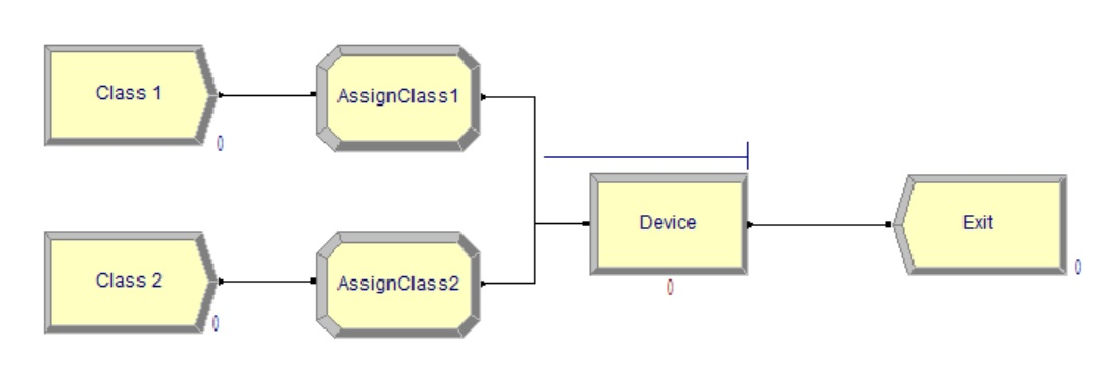
\includegraphics[width=1\linewidth]{model_Arena}}
\caption{Модель СМО в системе Arena}
\label{ris:model_Arena}
\end{figure} %вставить ссылку на рисунок

\begin{figure}[h] %определить место рисунка в тексте
\center{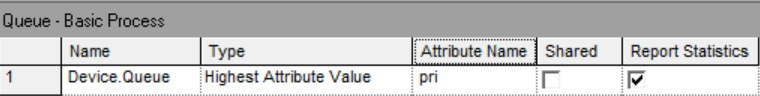
\includegraphics[width=0.7\linewidth]{queue_pri}}
\caption{Настройка очереди с относительными приоритетами}
\label{ris:queue_pri}
\end{figure} %вставить ссылку на рисунок

\begin{figure}[h] %определить место рисунка в тексте
\center{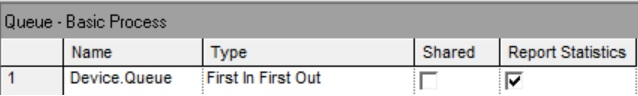
\includegraphics[width=0.7\linewidth]{queue}}
\caption{Настройка очереди с бесприоритетной дисциплиной обслуживания}
\label{ris:queue}
\end{figure} %вставить ссылку на рисунок

\subsection{Замеры времени моделирования в Arena}
Количество экспериментов (12) для аналогично предыдущим системам. Так как время работы системы заметно больше, чем в AnyLogic и GPSS World, то сделаем прогоны с количеством заявок, равным 100.000, 500.000 и 1.000.000. 

\begin{table}[h!]
\caption{Результаты измерений СМО с ДО БП}
\begin{tabular}{|c|c|c|c|c|c|c|c|c|c|}
\hline
 & \multicolumn{3}{|c|}{100.000} & \multicolumn{3}{|c|}{500.000} & \multicolumn{3}{|c|}{1.000.000} \\
\hline
 & 0.1+0.1 & 0.3+0.3 & 0.48+0.48 & 0.1+0.1 & 0.3+0.3 & 0.48+0.48 & 0.1+0.1 & 0.3+0.3 & 0.48+0.48 \\
\hline
1 замер & 6 & 5 & 6 & 25 & 28 & 29 & 55 & 55 & 52   \\
\hline
2 замер & 5 & 5 & 6 & 27 & 27 & 27 & 54 & 57 & 58   \\
\hline
3 замер & 5 & 5 & 6 & 26 & 27 & 29 & 51 & 56 & 53  \\
\hline
4 замер & 5 & 5 & 6 & 28 & 28 & 29 & 51 & 56 & 57  \\
\hline
Ср.знач. & 5.25 & 5 & 6 & 26.5 & 27.5 & 28.5 & 52.75 & 56 & 55   \\
\hline
\end{tabular}
\end{table} 

\begin{table}[h!]
\caption{Доверительные интервалы измерений СМО с ДО БП}
\begin{tabular}{|c|c|c|c|c|c|}
\hline
 Количество заявок & Среднее значение & С.к.о. & Дов. вероятность & Дов. интервал & Результат\\
\hline
100.000 & 5.42 & 0.42 & 95\% & 1.06 & 5.42 ± 1.06 \\
\hline
500.000 & 27.50 & 0.82 & 95\% & 2.03 & 27.50 ± 2.03 \\
\hline
1.000.000 & 54.58 & 1.36 & 95\% & 3.38 & 54.58 ± 3.38 \\
\hline
\end{tabular}
\end{table} 

\begin{table}[h!]
\caption{Результаты измерений СМО с ДО ОП}
\begin{tabular}{|c|c|c|c|c|c|c|c|c|c|}
\hline
 & \multicolumn{3}{|c|}{100.000} & \multicolumn{3}{|c|}{500.000} & \multicolumn{3}{|c|}{1.000.000} \\
\hline
 & 0.1+0.1 & 0.3+0.3 & 0.48+0.48 & 0.1+0.1 & 0.3+0.3 & 0.48+0.48 & 0.1+0.1 & 0.3+0.3 & 0.48+0.48 \\
\hline
1 замер &  5 & 5 & 6 & 26 & 27 & 28 & 51 & 53 & 53    \\
\hline
2 замер &  5 & 5 & 6 & 27 & 27 & 27 & 53 & 53 & 56 \\
\hline
3 замер &   5 & 5 & 5 & 26 & 28 & 27 & 52 & 52 & 54  \\
\hline
4 замер &  5 & 6 & 5 & 28 & 26 & 28 & 54 & 53 & 53 \\
\hline
Ср.знач. &  5 & 5.25 & 5.5 & 26.75 & 27 & 27.5 & 52.5 & 52.75 & 54  \\
\hline
\end{tabular}
\end{table} 

\begin{table}[h!]
\caption{Доверительные интервалы измерений СМО с ДО ОП}
\begin{tabular}{|c|c|c|c|c|c|}
\hline
 Количество заявок & Среднее значение & С.к.о. & Дов. вероятность & Дов. интервал & Результат\\
\hline
100.000 & 5.25 & 0.20 & 95\% & 0.51 & 5.25 ± 0.51 \\
\hline
500.000 & 27.08 & 0.31 & 95\% & 0.77 & 27.08 ± 0.78 \\
\hline
1.000.000 & 53.08  & 0.66 & 95\% & 1.63 & 53.08 ± 1.64 \\
\hline
\end{tabular}
\end{table} 

\section{Система MATLAB + Simulink}
\subsection{Описание системы }
MATLAB — это высокоуровневый язык и интерактивная среда для программирования, численных расчетов и визуализации результатов. С помощью MATLAB можно анализировать данные, разрабатывать алгоритмы, создавать модели и приложения. 

Программа Simulink является расширением программного пакета MATLAB. Simulink - это графическая среда имитационного моделирования, позволяющая при помощи блок-диаграмм в виде направленных графов, строить динамические модели, включая дискретные, непрерывные и гибридные, нелинейные и разрывные системы. Simulink является достаточно самостоятельным инструментом MATLAB и при работе с ним совсем не требуется знать сам MATLAB и остальные его приложения. С другой стороны доступ к функциям MATLAB и другим его инструментам остается открытым и их можно использовать в Simulink. 

Для реализации дискретно-событийного моделирования в среде Simulink используется компонента SimEvents. С помощью SimEvents можно моделировать и проектировать распределенные системы управления, аппаратные конфигурации, сети передачи и сбора информации для аэрокосмических, автомобильных, электронных и других приложений. Можно также моделировать событийно-управляемые процессы, такие например, как стадии производственного процесса для определения потребностей в ресурсах и оценки узких мест производства. SimEvents и Simulink создают интегрированную среду для моделирования гибридных динамических систем, содержащих непрерывные компоненты и компоненты с дискретными событиями и дискретным временем. 

\subsection{Создание моделей СМО в Simulink}
Для открытия библиотек SimEvents нужно ввести в командной строке simeventslib. Выберем из раздела Generators (подраздел Entity Generators - генераторы сущностей) два блока Time-Based Entity Generator для генерации сущностей, из раздела Queues блок FIFO Queue для хранения сущностей в очереди (бесприоритетная дисциплина обслуживания), из раздела Servers - блок Single Server для обслуживания сущностей, из раздела SimEvents Sinks - блок Entity Sink для удаления сущностей и четыре блока Signal Scope для отображения информации о ходе моделирования. Емкость очереди примем бесконечной (inf). Времена обслуживания задаются через сигнальный порт t (Service time from - Signal port t) блоком Event Based Random Number. Так как линии для связи сущностей нельзя разветвлять, а в очередь у нас попадает два класса заявок, воспользуемся блоком Path Combiner. В результате в окне модели будет отображаться следующая картина (рис 4.5).
\begin{figure}[h] %определить место рисунка в тексте
\center{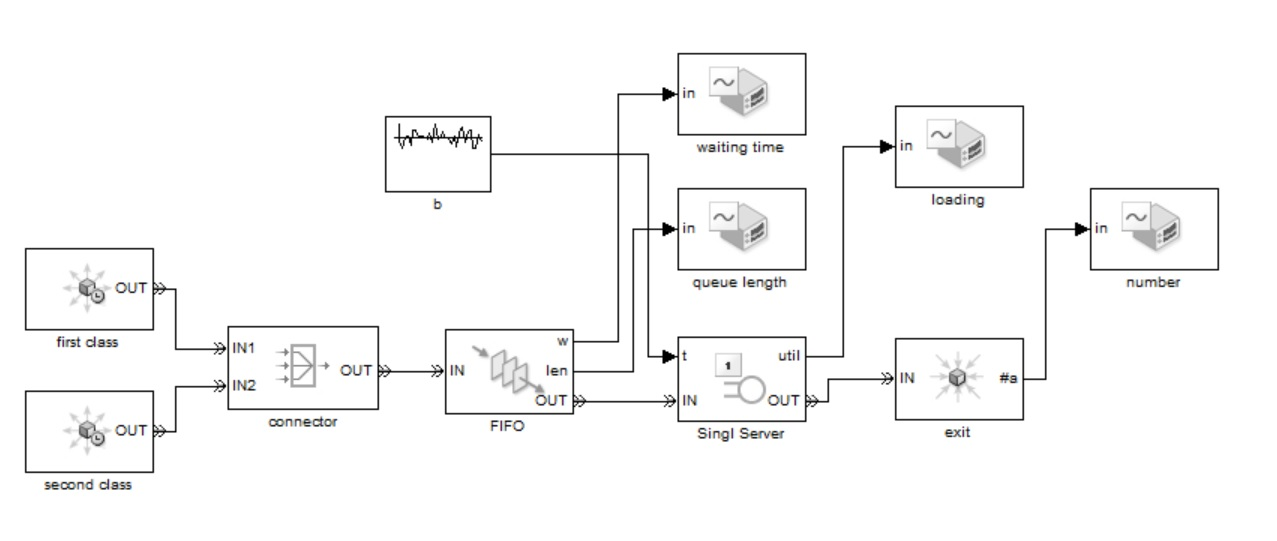
\includegraphics[width=1\linewidth]{matlab_fifo}}
\caption{Модель СМО с ДО БП в MATLAB}
\label{ris:matlab_fifo}
\end{figure} %вставить ссылку на рисунок

Чтобы построить модель с ДО ОП, мы должны задать переменную, которая будет определять приоритет заявки. Для этого воспользуемся двумя блоками Set Attribute, затем с помощью команды добавления (Add) создадим переменную ServiceTime и зададим первому и второму классу заявок приоритеты 1 и 2 соответственно. Для хранения сущностей в очереди изменим блок на Priority Queue из раздела Queues, а в параметрах зададим ёмкость (capacity) равной бесконечности (inf) и название нашей переменной ServiceTime для определения приоритета. Остальная модель остаётся без изменений. Окончательную модель для СМО с ДО ОП можно увидеть на рис. 4.6.
\begin{figure}[h] %определить место рисунка в тексте
\center{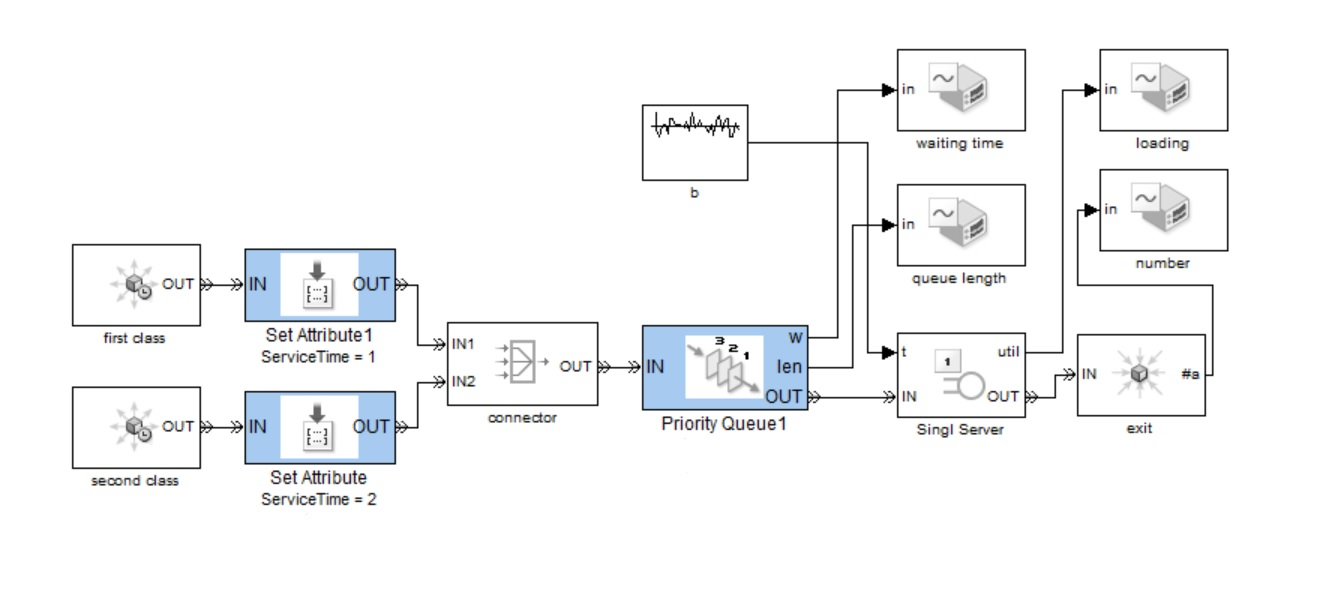
\includegraphics[width=1\linewidth]{matlab_pri}}
\caption{Модель СМО с ДО ОП в MATLAB}
\label{ris:matlab_pri}
\end{figure} %вставить ссылку на рисунок

\subsection{Замеры времени моделирования в Simulink}
\begin{table}[h!]
\caption{Результаты измерений СМО с ДО БП}
\begin{tabular}{|c|c|c|c|c|c|c|c|c|c|}
\hline
 & \multicolumn{3}{|c|}{100.000} & \multicolumn{3}{|c|}{500.000} & \multicolumn{3}{|c|}{1.000.000} \\
\hline
 & 0.1+0.1 & 0.3+0.3 & 0.48+0.48 & 0.1+0.1 & 0.3+0.3 & 0.48+0.48 & 0.1+0.1 & 0.3+0.3 & 0.48+0.48 \\
\hline
1 замер &  &  &  &  &  &  &  &  &   \\
\hline
2 замер &   &  &  &  &  &  &  &  &    \\
\hline
3 замер & &  &  &  &  &  &  &  &   \\
\hline
4 замер &   &  &  &  &  &  &  &  &  \\
\hline
Ср.знач. &   &  &  &  &  &  &  &  &   \\
\hline
\end{tabular}
\end{table} 

\begin{table}[h!]
\caption{Доверительные интервалы измерений СМО с ДО БП}
\begin{tabular}{|c|c|c|c|c|c|}
\hline
 Количество заявок & Среднее значение & С.к.о. & Дов. вероятность & Дов. интервал & Результат\\
\hline
100.000 &  &  & 95\% & &  ±  \\
\hline
500.000 &  &  & 95\% &  &  ±  \\
\hline
1.000.000 &  &  & 95\% & &  ±  \\
\hline
\end{tabular}
\end{table} 

\begin{table}[h!]
\caption{Результаты измерений СМО с ДО ОП}
\begin{tabular}{|c|c|c|c|c|c|c|c|c|c|}
\hline
 & \multicolumn{3}{|c|}{100.000} & \multicolumn{3}{|c|}{500.000} & \multicolumn{3}{|c|}{1.000.000} \\
\hline
 & 0.1+0.1 & 0.3+0.3 & 0.48+0.48 & 0.1+0.1 & 0.3+0.3 & 0.48+0.48 & 0.1+0.1 & 0.3+0.3 & 0.48+0.48 \\
\hline
1 замер &   &  &  &  &  &  &  &  &     \\
\hline
2 замер &  &  &  &  &  &  &  &  &   \\
\hline
3 замер &   &  &  &  &  &  &  &  &    \\
\hline
4 замер &   &  &  &  &  &  &  &  &  \\
\hline
Ср.знач. &   &  &  &  &  &  &  &  &   \\
\hline
\end{tabular}
\end{table} 

\begin{table}[h!]
\caption{Доверительные интервалы измерений СМО с ДО ОП}
\begin{tabular}{|c|c|c|c|c|c|}
\hline
 Количество заявок & Среднее значение & С.к.о. & Дов. вероятность & Дов. интервал & Результат\\
\hline
100.000 &  & & 95\% &  &  ±  \\
\hline
500.000 &  &  & 95\% &  &  ±  \\
\hline
1.000.000 &   & & 95\% &  &  ±  \\
\hline
\end{tabular}
\end{table} 

\section{Сравнение}
Сравним полученные результаты для разных СМО в системах GPSS World и AnyLogic: 

\begin{table}[h!]
\caption{Сравнение СИМ ДО БП}
\begin{tabular}{|c|c|c|c|c|}
\hline
 & GPSS World & AnyLogic 7.1  &  Arena & MATLAB\\
\hline
1.000.000 & 3.33 ± 0.30 & 15.69 ± 1.01 & 54.58 ± 3.38 &\\
\hline
5.000.000 & 17.25 ± 0.51 & 64.13 ± 3.37 & & \\
\hline
10.000.000 & 35.75 ± 1.5 & 117.15 ± 3.88 & & \\
\hline
\end{tabular}
\end{table} 

\begin{table}[h!]
\caption{Сравнение СИМ ДО ОП}
\begin{tabular}{|c|c|c|c|c|}
\hline
 & GPSS World & AnyLogic 7.1 & Arena & MATLAB \\
\hline
1.000.000 & 3.83 ± 0.59 & 14.98 ± 0.70 & 53.08 ± 1.64 & \\
\hline
5.000.000 & 18.50 ± 0.51 & 66.31 ± 1.87 &  & \\
\hline
10.000.000 & 37.33 ± 0.30 & 110.60 ± 2.57&   &\\
\hline
\end{tabular}
\end{table} 

Как мы видим, система GPSS World работает в несколько раз быстрее, чем система AnyLogic 7.1 и Arena при равных условиях: одинаковом количестве характеристик и без визуализации моделирования. Но с другой стороны, хотя GPSS работает быстрее, в программе на языке GPSS достаточно сложно представить непосредственно процессы обработки данных на уровне алгоритмов, кроме того, модель представляет собой программу, а значит не имеет графической интерпретации, что затрудняет процесс разработки модели и снижает наглядность модели в целом.

Однако, для каждой системы в отдельности разница между полученными доверительными интервалами времени для бесприоритетной дисциплины обслуживания и дисциплины с относительными приоритетами несущественна.
\chapter{Выводы по работе}
\end{document}